\section{Inleiding}

De term \emph{computernetwerk} bestaat uit twee woorden: ``computer'' en ``netwerk.''
Wikipedia definiëert een \emph{computer} als een ``apparaat waarmee gegevens volgens formele procedures verwerkt kunnen worden.''
Dat is echter een nogal vage definitie.
Gelukkig hebben we allemaal wel een goed idee van wat een computer is: een laptop of desktop computer.
Maar ook servers, netwerkprinters, tablets en gsm-toestellen zijn volwaardige computers.
Meer nog, tegenwoordig zit er zelfs een computer in je auto of het mengpaneel van een muziekinstallatie!

Een \emph{netwerk} is, volgens Wikipedia, een ``systeem voor communicatie tussen twee of meer computers.''
Hier denken we dan misschien meteen aan het wireless netwerk of de ``internetkabel'' op kantoor of bij je thuis;
maar je kan ook netwerken maken met infrarood (IrDA), bluetooth of 5G.
Glasvezel, ADSL en coax zijn ook voorbeelden van computernetwerken.



\subsection{Netwerkprotocollen}

Een protocol is, om weeral Wikipedia te citeren, een ``gedragsovereenkomst, meestal in de vorm van een aantal uit te voeren stappen.''
Het vormt dus een set regels waar twee computers zich aan willen houden, als ze met elkaar willen communiceren.
We kunnen dit vergelijken met enkele gedragsregels uit het dagelijks leven.
Als je een nieuw persoon ontmoet, schud je elkaar de hand en stel je jezelf kort voor.%
  \footnote{Covid-19 heeft er voor gezorgd dat er een ander protocol gebruikt wordt in deze (en vele andere) situatie.}
In de klas zwijgt iedereen zodat de docent zijn uitleg kan doen.
Als je een vraag wil stellen, steek je de hand omhoog en wacht je tot de docent stopt met praten en jou aanduidt zodat jij aan het woord mag.
Als je de koning mag ontmoeten, moet je een heel nieuw protocol leren voor de interactie.

Computernetwerken gebruiken ook verschillende protocollen.
Enkele protocollen die we in deze cursus (kort) zullen behandelen, zijn
IPv4 en IPv6, TCP en UDP, Ethernet en ARP.
Enkele protocollen die niet meer gebruikt worden in computernetwerken, zijn IPX, SPX en AppleTalk.



\subsection{Evolutie in netwerken}

De eerste \emph{mainframes} stammen uit de jaren 50.
De gegevens werden oorspronkelijk ingevoerd met gegevensdragers als ponskaarten, ponsbanden en magneetbanden.
In de jaren 70 werden op enige schaal terminals aan mainframes aangesloten, aanvankelijk schrijfmachineterminals en later ook beeldschermen.

In 1971 werd ALOHAnet in gebruik genomen in Hawaï.
Dit was het eerste draadloos computernetwerk.
In 1973--74 werd Ethernet ontwikkeld op basis van dit draadloos netwerk.
Ethernet gebruikte eerst thicknet (1982), daarna thinnet (1983), en vervolgens twisted pair (1984).
Concurrerende protocollen waren Token Ring (1984) en FDDI (1987).
Begin jaren 90 kwamen de Ethernetswitches en verdrong Ethernet vrij snel alle andere protocollen.



\subsection{Netwerktopologieën}

De meest eenvoudige topologie is een point-to-pointverbinding tussen twee computers door beide computers rechtstreeks met elkaar te verbindinen met een kabel.
Deze topologie schaalt echter niet goed.
Enkele voorbeelden zijn een seriële kabel, een UTP-kabel, of eeninfraroodverbinding.

Thick- en thinnet gebruiken beide een fysieke busstructuur waarbij alle computers op één lange kabel geprikt worden.
Beide standaarden gebruiken coax (echter van een andere dikte, vandaar de namen) maar beide gebruiken een andere manier om de computers met het netwerk te verbinden.
Thicknet gebruikt ``vampire taps'' en een \emph{drop cable} terwijl thinnet BNC-koppelstukken gebruikt.%
   \footnote{Er was ook een N-connector beschikbaar voor Thicknet maar deze werd blijkbaar amper gebruikt (\href{http://www.mattmillman.com/projects/10base5/}{bron}).}

Hoewel Token Ring een fysieke stertopologie heeft -- met een centrale media access unit (MAU) -- vormen de kabels een logische ringtopologie.
Hubs en switches vormen ook een fysieke stertopologie.
Een hub werkt functioneel zoals thinnet en vormt aldus een logische busstructuur terwijl een switch als een reeks logische point-to-pointverbindingen werkt.

Een \emph{full mesh} netwerk is een netwerk waarbij elk toestel met elk ander toestel verbonden is door middel van point-to-pointverbindingen.
Een \emph{partial mesh} netwerk is een netwerk waarbij een deel van de directe verbindingen van een full mesh ontbreken.

\subsection{Het OSI-model en het TCP/IP-model}

Het OSI-model is een conceptueel model voor netwerkcommunicatie.
Het werd als theoretisch model ontwikkeld met de bedoeling dat de praktijk zich aan dit model aan zou passen.
Het TCP/IP-model is een alternatief protocol dat gebaseerd is op de protocollen die al in de praktijk gebruikt werden.

\begin{table}[htp]
   \centering
   \begin{tabular}{rll}
   %\toprule
     & \textit{OSI-model} & \textit{TCP/IP-model} \\[1ex]
   %\midrule
   \textit{7} & application & \multirow{3}{*}{\textcolor{spot1}{application}} \\
   \textit{6} & presentation & \\
   \textit{5} & session & \\[1ex]
   \textit{4} & \textcolor{spot1}{transport} & transport \\[1ex]
   \textit{3} & \textcolor{spot1}{network} & internet \\[1ex]
   \textit{2} & \textcolor{spot1}{data link} & \multirow{2}{*}{link} \\
   \textit{1} & \textcolor{spot1}{physical} & \\
   %\bottomrule
   \end{tabular}
   \caption{De zeven lagen van het OSI-model en de vier lagen van het TCP/IP-model.
   De vijf lagen van het hybride model zijn in kleur weergegeven.}
   \label{tab:osi-model}
\end{table}

Deze modellen hebben weinig praktisch nut maar kunnen wel helpen met het gestructureerd opsporen en oplossen van netwerkproblemen.
Afhankelijk van het probleem kan je ofwel op laag~7 (de applicatie) beginnen met troubleshooten, ofwel op laag~1 (de bekabeling), ofwel in het midden op laag~3 (het netwerk).
Onderstaand vind je voor de vijf lagen van het hybride model enkele zaken die onderzocht kunnen worden.

\begin{description}
\item[application]
   Controleer de configuratie van de applicatie zelf.
   Dit is aan de applicatie- of systeembeheerders en niet aan de netwerkbeheerder.
\item[transport]
   Controleer firewallconfiguraties en of de service (applicatie) wel gestart is op de server.
   Je kan met behulp van \cmd{telnet} testen of de applicatie bereikbaar is.
\item[network]
   Verifiëer met behulp van \cmd{ping} en \cmd{traceroute} of de twee computers elkaar kunnen bereiken.
   De output van \cmd{traceroute} geeft een indicatie hoe de pakketjes doorheen het netwerk gaan.
   Dit kan je best in beide richtingen controleren aangezien \emph{asymetrisch} netwerkverkeer mogelijk is en mogelijk voor problemen kan zorgen.
\item[data link]
   Op het lokale netwerk moet je zaken zoals Spanning-tree protocol (STP) en VLAN-configuraties nakijken.
   Zaken zoals DHCP snooping, dynamic ARP inspection (DAI) en port security kan je hier ook nakijken.
\item[physical]
  Controleer bekabeling, connectors, interface errors en, in het geval van wifi, mogelijke storingsbronnen.
\end{description}

De verschillende lagen vinden we ook terug als we de verschillende stappen doorlopen die computers doorlopen om met elkaar te communiceren.




\subsection{Soorten communicatie}

Op een netwerk bestaan er vier soorten van communicatie.
We spreken over \emph{unicast} als één computer met één andere computer communiceert over het netwerk, bijvoorbeeld als je met SSH een computer vanop afstand configureert.
Een tweede soort van communicatie is \emph{broadcast}: een computer communiceert met alle computers binnen een bepaald netwerk.
Voorbeelden hiervan zijn DHCP (\vref{sec:dhcp}) en ARP (\vref{sec:arp}).

Als een computer met verschillende, maar niet alle, computers wil communiceren, spreken we van \emph{multicast}.
Denk hierbij bijvoorbeeld aan digitale tv.
Enkel de tv-toestellen die een bepaalde zender hebben opstaan, willen die beelden ontvangen.

Tot slot is er ook nog \emph{anycast}, hetgeen niet expliciet benoemd worden in IPv4 maar wel benadrukt wordt bij IPv6.
In weze is dit hetzelfde als unicast maar door slim te routeren binnen het netwerk, communiceer je altijd met de dichtst bijzijnde server.
Wil je bijvoorbeeld een groot bestand downloaden van het Internet, dan zal dit sneller gaan als je dit kan downloaden van een server in je eigen land dan van een server in een ander continent.
Anycast is de methode die \emph{content delivery networks} (CDN) zo interessant maken en die gebruikt worden om de DNS root servers over de gehele wereld beschikbaar te maken (\vref{sec:dns}).

In deze cursus gaan we niet dieper in op multicast of anycast.



\subsection{Communicatie tussen computers}

Nemen we als voorbeeld een computer, de \emph{client}, die een webpagina op wil halen van een andere computer, de \emph{server} (\vref{fig:client-server}).
Het protocol dat hier voor gebruikt wordt, heet hypertext transfer protocol (HTTP).
De client verstuurt een HTTP \emph{request} en de server antwoordt met een HTTP \emph{response}.

De request bevat de volgende data.
\begin{verbatim}
GET /index.html HTTP/1.1
Host: www.example.com
\end{verbatim}

\begin{figure}
   \centering
   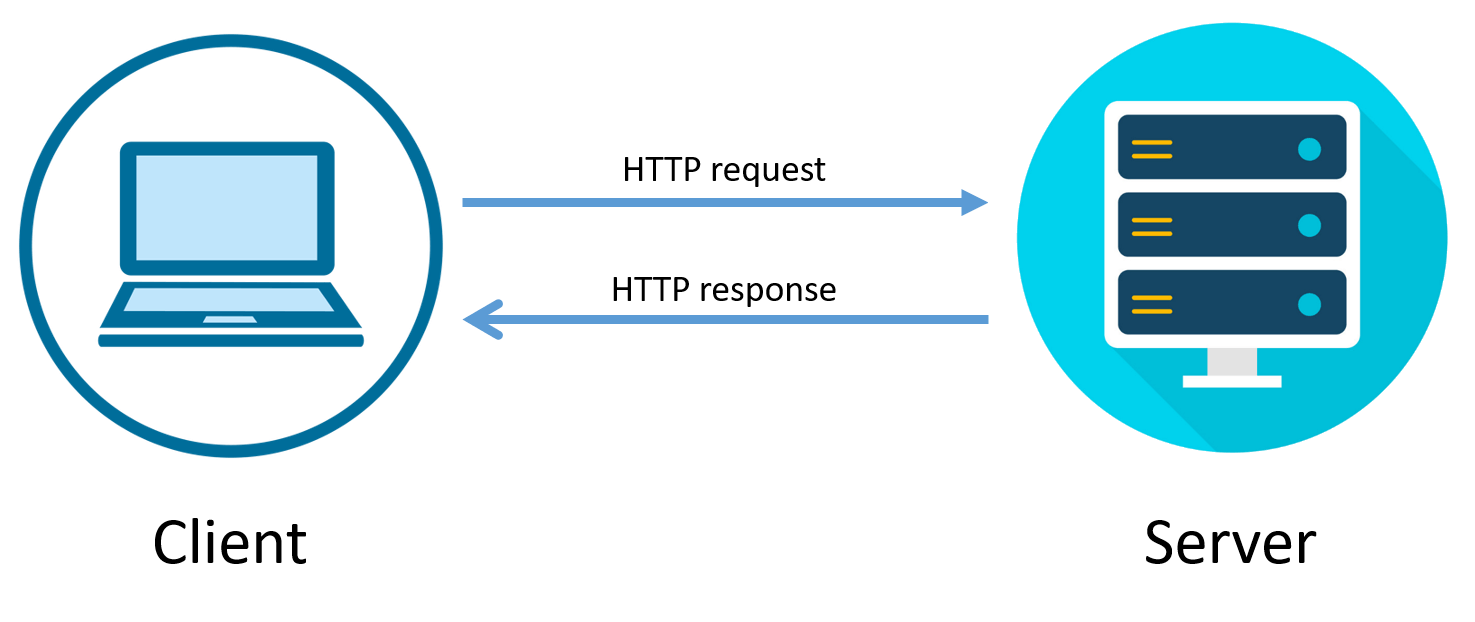
\includegraphics[width=.65\textwidth]{images/http-request.png}
   \caption{Een client vraagt een webpagina op bij eeen webserver en gebruikt voor deze communicatie HTTP}
   \label{fig:client-server}
\end{figure}

Het antwoord van de server bevat enerzijds de HTTP-data die het protocol vereist en anderzijds de gevraagde webpagina.
In dit geval bevat de gevraagde pagina HTML-code.
\begin{verbatim}
HTTP/1.1 200 OK
Content-Type: text/html; charset=UTF-8
Content-Length: 155
Server: Apache/1.3.3.7 (Unix) (Red-Hat/Linux)

<html>
  <head><title>An Example Page</title></head>
  <body><p>Hello World!</p></body>
</html>
\end{verbatim}

Dit ogenschijnlijk eenvoudig voorbeeld roept toch meerdere vragen op.
\begin{enumerate}
\item Hoe kunnen we de server bereiken?
\item Voor welke applicatie is de data bestemd?
\item Hoe versturen we heel veel data?
\item Wat doen we als er iets mis gaat?
\end{enumerate}



\subsubsection{Hoe kunnen we de server bereiken?}
In de adresbalk van de browser vullen we de \emph{domeinnaam} van de website in die we willen bereiken, bijvoorbeeld \url{www.example.com}.
Deze domeinnaam vinden we ook terug in de Host header van de HTTP request.
Omdat computers met elkaar communiceren door middel van IP-adressen, moet deze domeinnaam eerst omgezet worden in een IP-adres.
Dit gebeurt met behulp van het Domain Name System (DNS).

\subsubsection{Voor welke applicatie is de data bestemd?}
Als pakketjes aankomen op een server of client computer, moet het besturingssysteem weten voor welke applicatie ze bestemd zijn.
Bevatten de pakketjes een email bestemd voor Outlook of een gif van een kat die in de browser getoond moet worden?
Elk programma dat communiceert op het netwerk krijgt een poortnummer toegewezen.
Deze poortnummers worden meegestuurd in de pakketjes zodat de computers steeds weten voor welke applicatie de pakketjes bestemd zijn.
We leren meer over deze poortnummers als we TCP en UDP bespreken.

\subsubsection{Hoe versturen we heel veel data?}
Als we een groot document door willen sturen, reist de vraag of we dit document als één geheel kunnen sturen, of moeten opsplitsen in kleine stukjes om vervolgens deze kleine stukjes afzonderlijk te versturen.
We zullen merken dat er technische beperkingen zijn die de maximale grootte van een pakket bepalen op sommige netwerken.
Het is soms dus noodzakelijk om grote bestanden op te splitsen en als kleine stukjes te versturen.

Als we een groot bestand opsplitsen in twintig kleine stukjes en deze afzonderlijk versturen, moet de ontvanger van deze twintig pakketjes er wel in slagen om ze alle twintig terug samen te puzzelen tot één geheel.
De ontvanger moet ook zeker dat dat hij alle stukjes ontvangen heeft.
Het is belangrijk dat hij weet dat de verzender twintig pakketjes verstuurd heeft in plaats van eenentwintig.

Deze vraagt hangt ook samen met de volgende vraag.

\subsubsection{Wat doen we als er iets mis gaat?}
Pakketjes kunnen verloren gaan of er kunnen ``beschadigingen'' optreden in een pakketje (een ``1'' kan een ``0'' worden of omgekeerd).
Pakketjes kunnen in de verkeerde volgorde aankomen.
Dit zijn uitdagingen die TCP en UDP wel (of bewust niet) oplost.




\subsection{Encapsulatie en decapsulatie}

We gaan nu terug naar de computer die een HTTP request stuurt naar de web server.
De computer heeft een DNS request uitgestuurd voor de domeinnaam www.example.com en kreeg het IP-adres 192.168.1.102.
De HTTP request wordt nu ``ingepakt'' in een TCP-pakket (\vref{fig:transmit-data}).
Dit ``inpakken'' (\emph{encapsulation}) is niet meer dan wat extra data toe te voegen, ofwel voor ofwel na de andere data.
TCP voegt onder andere de nodige poortnummers toe.


\begin{figure}
   \centering
   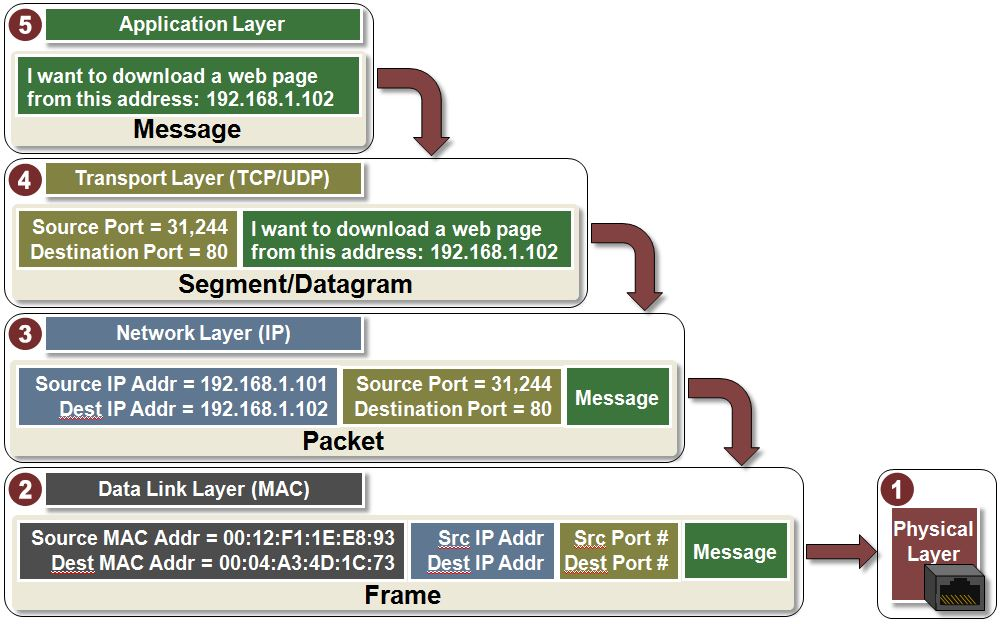
\includegraphics[width=\textwidth]{images/transmit_data.jpg}
   \caption{Elk protocol voegt een eigen header toe aan het pakket}
   \label{fig:transmit-data}
\end{figure}

Vervolgens wordt het pakket doorgegeven aan IP.
Deze voegt de source en destination IP-adressen toe.
Vervolgens voegt Ethernet een header toe met source en destination MAC-adressen waarna het pakket door de netwerkkaart het netwerk wordt opgestuurd.
Dit is de physical layer.


%\begin{frame}{Communicatie gebeurt tussen lagen onderling}
%\begin{center}
%\includegraphics<presentation>[width=\textwidth]{images/tcpip_5_layer_overview.png}
%\includegraphics<article>[width=.65\textwidth]{images/tcpip_5_layer_overview.png}
%\end{center}
%Bron: \url{https://microchipdeveloper.com/}
%\end{frame}
%

